%-----------CHAPTER 7-------------------------------------------
%-------Ringdown Search----------------------------------------
\chapter{Data Analysis for Black Hole Ringdowns}
\label{chap:ringdowns}


\begin{figure}[!h]
\centerline{\includegraphics[angle=0,width=6.5in]{Figures/Chap1/GRB-DestroyStar.jpg}}
\end{figure}
\clearpage


This chapter describes an analysis done of the data from the second LIGO Science
Run (called S2) to look for damped sinusoid signals such as are expected from
the ringdown of black hole quasi-normal modes (see Section~\ref{sec:Ringdowns}). The
analysis was carried out over all times during which both of the 4 km interferometers were
running in their nominal data taking state.

This was an exploratory analysis, whose purpose was to answer the following questions:

\begin{itemize}

\item What is the sensitivity of the interferometers to ringdowns?

\item How much worse is the sensitivity than that of an interferometer with
      Gaussian noise of the same strain spectral density?

\item What specific things cause the sensitivity to be degraded?

\item What improvements can be made to the standard matched filter search
      as it applies to ringdowns? 

\end{itemize} 
%------------------------------------------------------------------------------
\section{Overview of the Method}

This section describes the steps involved in producing ringdown triggers from
the raw data. This part of the analysis
is similar to the analysis done by the LIGO 
Inspiral~\cite{S1:Inspiral} group.

The ringdown signals are searched for using a matched filtering code. The
matched filter templates are damped cosine waveforms which span the frequency
and quality factor (Q) space over the sensitive band of the detector and among
the Q's expected for Kerr black holes.

All of the code up to and including the trigger generation was taken from
the LIGO Algorithm Library (LAL)~\footnote{
\href{http://www.lsc-group.phys.uwm.edu/lal/}{http://www.lsc-group.phys.uwm.edu/lal/}}. 
It is C code compiled as a stand-alone executable to run on UNIX from the command line. 
For this analysis, it was sufficient to individually launch the jobs
on $\sim$10 CPU's at a time. It took $\sim$50 hours to run
the full 300 hour S2 data set for 2 interferometers using $\sim$350
templates per interferometer.

The post-processing is all done using 
MATLAB~\footnote{
\href{http://www.mathworks.com}{http://www.mathworks.com}} scripts.


\begin{figure}[!h]
\centerline{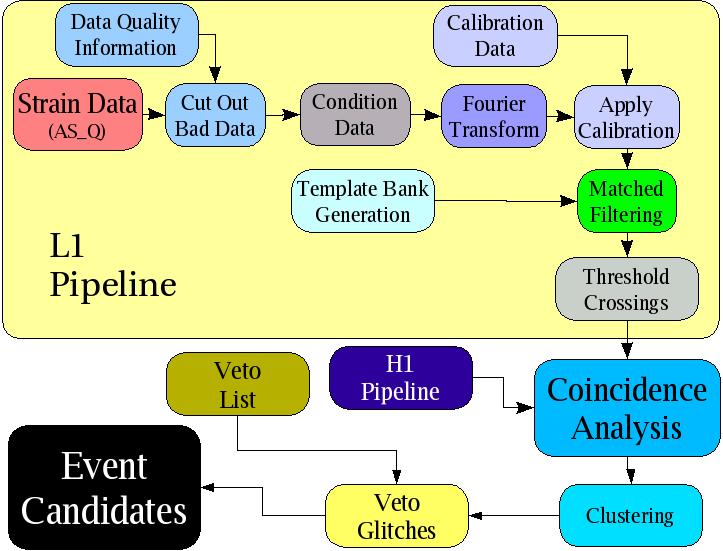
\includegraphics[angle=0,width=6.5in]{Figures/Chap7/Pipeline.png}}
\caption[Ringdown Pipeline]{The analysis pipeline.}
\label{fig:pipeline}
\end{figure}

\subsection{Matched Filtering}

The front end of the analysis pipeline uses matched filtering to produce an initial
set of ringdown triggers. Matched filtering is a commonly used technique to look
for signals of a known waveform in a noisy data stream~\cite{Bruce:MF}. A
matched filter is the optimum linear filter for the detection of a known
waveform.

We can write the calibrated detector output as a time series, $h(t)$, which is 
the sum of the signal, $s(t)$ and some noise, $n(t)$:

\begin{equation}
h(t) = s(t) + n(t)
\end{equation}
The Fourier transform of the template is

\begin{equation}
s(f) = \int\limits_{-\infty}^{\infty} s(t) e^{-2 \pi i f t} \, dt
\end{equation}
The matched filter output is

\begin{equation}
x(t) = 4 \int\limits_{0}^{\infty} \frac{s(f) h(f)}{S_n(f)} e^{2 \pi i f t} \, df
\label{eq:MF}
\end{equation}
The matched filter variance is given by

\begin{equation}
\sigma^2 = 4 \int\limits_{0}^{\infty} \frac{s(f)^2}{S_n(f)}\, df
\end{equation}
Thresholding on the signal-to-noise ratio (SNR),

\begin{equation}
\rho = x/\sigma
\end{equation}
is the optimal detection statistic for stationary, Gaussian
detector noise \cite{Jolien:40m}.

\begin{figure}[!h]
\centerline{\includegraphics[angle=0,width=6.5in]{Figures/Chap7/templatespacing_f_Q.png}}
\caption[Template Spacing (f,Q)]{Template spacing for maximum mismatch $\rightarrow$ 5\% in SNR. 
         Each dot represents one template.}
\label{fig:templates_f_Q}
\end{figure}

\begin{figure}[!h]
\centerline{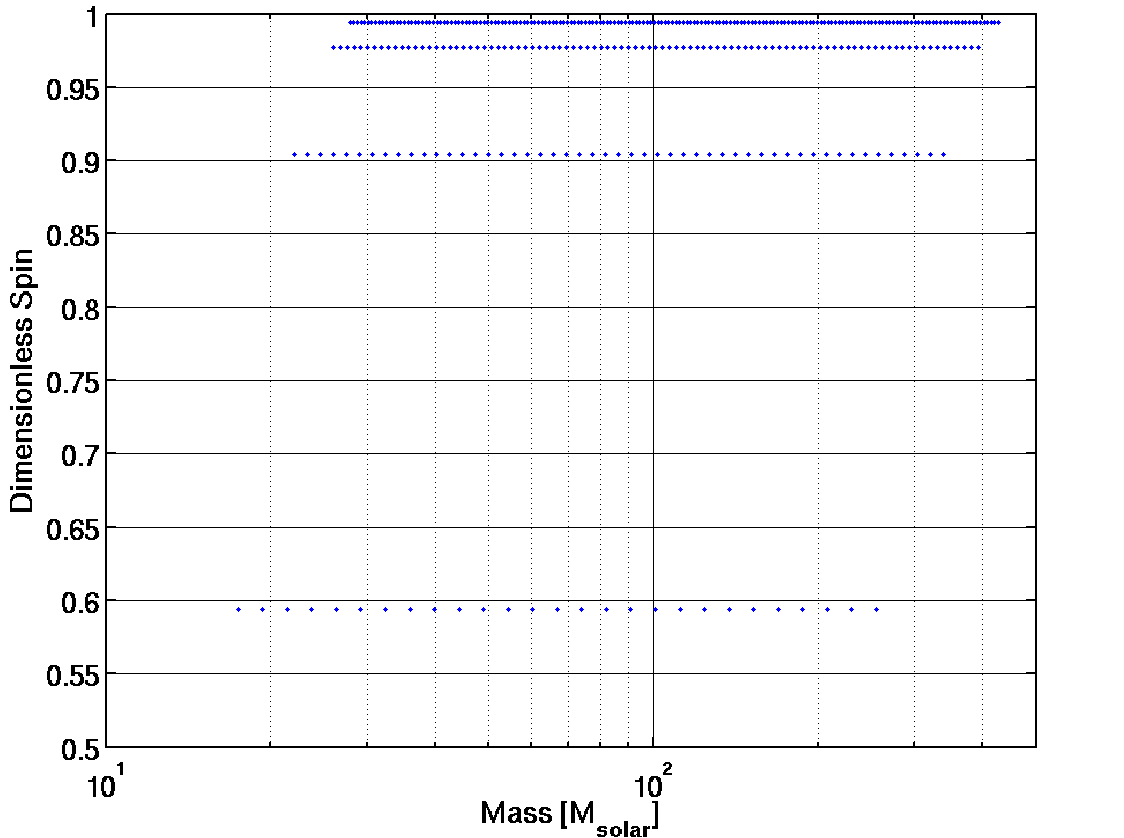
\includegraphics[angle=0,width=6.5in]{Figures/Chap7/templatespacing_M_a.png}}
\caption[Template Spacing (M,a)]{Template spacing in the (Mass, Spin) plane. These are the
                          same templates plotted in Figure~\ref{fig:templates_f_Q} 
                          but in terms of black hole Mass and Spin}
\label{fig:templates_M_a}
\end{figure}



\subsubsection{FFT the data}

The data are Fourier transformed using the Fast Fourier Transform (FFT)
algorithm, which allows the matched filter output to be calculated by
using, of order N ln(N) operations. 

\subsubsection{Inverse power spectrum}

The power spectrum which is in the denominator of Equation~\ref{eq:MF}
is estimated in nearly the same way as Welch's method: By doing a 50\% 
overlapping average of 8 data segments of length 4 seconds, but in
this case a median average is done of the segments rather than a mean
to reduce the bias from one statistical outlier.

\subsubsection{Apply calibrations}

The interferometer response function is applied to the FFT of the data
and to the power spectrum estimate. The response function is generated as 
described in Chapter~\ref{chap:cal}.

\subsubsection{Choosing the event time}

The matched filter output due to a true ringdown signal will actually cross
the threshold several times in the few hundred milliseconds around the
real start time of the signal. 

The event is localized  by clustering all threshold crossings 
within a time, 
$\tau_{dur} = \frac{10 \, Q}{\pi f}$. The time with the maximum SNR is chosen
to be the event time.


\subsection{Data Conditioning}

Before the data are examined for signals, the raw time series must undergo
some conditioning. The data are whitened and decimated.

\subsubsection{Whitening}

The raw time series of the interferometer's output spans a very large dynamic range.
The purpose of whitening the data is to prevent data corruption.
Since the data are analyzed in the frequency domain, there is the possibility
of power bleeding into adjacent frequency bins. This effect is strongest
in some of the LIGO data streams where the amplitude of the noise at low 
frequencies is several orders of magnitude larger than the noise in the
gravitational wave signal band.

Without the suppression by the servo loop, the differential arm motion
would span $\sim$13 orders of magnitude on time-scales of 10's of
seconds. With the servo on the in-loop error point at the demodulator output 
spans $\sim$8 orders of magnitude. Although this is then 
further whitened by an analog filter to fit into the dynamic range of
the ADC, this analog filter is canceled by a digital filter before the
data channel, AS\_Q, is written to disk.

Numerous schemes have been proposed to do very detailed whitening of
the data including line removal~\cite{Hua:60Hz} and linear predictive
filtering~\cite{Shourov:LPF}. For
this analysis the data was merely high-passed to remove the large low
frequency power. 

The data are filtered with a fourth order infinite impulse response (IIR) 
Butterworth high pass filter. By filtering
the data backwards and forwards, the dispersion in the filter is canceled. 
The high pass filter frequency in this analysis was set at 60 Hz, 
just 5 Hz below the frequency of the lowest frequency template.


\subsubsection{Decimation}

The data is decimated from 16384 Hz down to 2048 Hz. This is done by first
filtering with a finite impulse response (FIR) low pass filter, then by
subtracting  a time shift to compensate for the linear $d\phi/df$ from
the FIR filter, and then downsampling by the appropriate amount. The
decimation essentially reduces the analysis time by the decimation factor
since the other overhead (data retrieval, writing to disk, etc.) does
not contribute significantly to the computation time.

Preliminary runs with a 4096 Hz sample rate revealed that the number
of triggers generated by L1 above $\sim$800 Hz is enormous; as
mentioned in Chapter~\ref{chap:noise} we know that this band was
dominated by oscillator-phase noise coupling in through the highly
non-stationary RF sideband imbalance. So in that respect this low
quality data is not surprising. The large number of triggers and the
poor sensitivity above 1 kHz motivated the choice of sample frequency.

With a 2048 Hz sample rate there is no information left above the new
Nyquist frequency, 1024 Hz. By choosing this band, we are cutting
out a range of low mass black holes. From Equation~\ref{eq:RD_f}
we see that this choice loses all masses below~$\sim$10~$M_{\astrosun}$.


\subsection{Template Bank Generation}
Methods have been developed to find the minimal number of templates required to
span the templates' parameter space and yet maintain a small loss in the SNR
\cite{Jolien:40m,Owen:templates,VIRGO:templates,TAMA:templates}. The basic
idea is to use the minimum number of filters possible without losing more
SNR than some small number. By calculating the SNR loss due to a small mismatch
of waveform parameters, one can define a metric in the coordinates
relevant for the waveform; in our case frequency and Q. Using the same method
as in \cite{Jolien:40m}:

\begin{equation}
ds^2 \approx \frac{1}{8}\frac{dQ^2}{Q^2} + \frac{1}{4}\frac{dQ}{Q}\frac{df}{f}
            + Q^2 \frac{df^2}{f^2}
\label{eq:TemplateMetric}
\end{equation}
where $ds^2$ is the SNR mismatch between two templates one at (f,Q) and one at
(f + df,Q + dQ). For this analysis we placed the templates by imposing the
requirement that the maximum SNR loss be $<$ 5\%.

The number of templates is:

\begin{equation}
N_{filters} \approx \frac{1}{4 \sqrt{2}} \, \frac{Q_{max}}{ds^{2}_{max}}
                \,    \ln{\frac{f_{max}}{f_{min}}}
\label{eq:Nfilters}
\end{equation}
For this analysis, $N_{filters} \simeq 350$. With the present computing speeds available
it takes only a few days to run the analysis for 350 hours of two interferometer
data on a dozen nodes. The main bottleneck in the analysis pipeline is still the
speed of the human data analyst and not the cleverness of the tiling algorithm.

Figures \ref{fig:templates_f_Q} and \ref{fig:templates_M_a} show the templates
spacing used in this analysis in the (f,Q) plane as well as the (M,a) plane.
Almost all of the templates bunch into the region of spin from 0.9 to 1.0
since there is not much variation of Q at low to mid spin values.

 

\section{Coincidence Analysis}
\label{sec:coin_anal}

The waveform from a true gravitational wave should be almost the same as seen by both
interferometers. So to reject false events, we demand some consistency in the
waveform parameters. Each trigger is labeled by five parameters: the start
time~($t_{start}$), the SNR, the peak strain~($h_{peak}$), the frequency~($f_{ring}$),
and the quality factor~($Q_{ring}$).


\subsection{Time}

The gravitational wave arrival time difference can be as much as
11 ms between sites. With a perfect detection algorithm and noiseless
data, we could use this number as our time coincidence cut. In reality,
there is some uncertainty in the arrival time due to having a low SNR and
that there is a small mismatch between the signal and the template. It is true
that we are ultimately limited by the sample time (0.5 ms) and the relative timing
error on the two data streams ($<$ 0.1 ms), but the residual timing errors
on the simulations did not reach this level.

We empirically determine the timing uncertainty by injecting a large number 
of events in software and measuring the resulting timing error 
(see Figure~\ref{fig:ParamEst}).

\subsection{Frequency}

Similar to the arrival time cut, we can do a frequency consistency check. To cut
down on the false alarm rate, it is desirable to have the smallest
frequency cut possible, maintaining a small false dismissal
probability.

\subsection{Q}

By the same reasoning, we would like to demand a tight Q cut. 

Since the same template bank is used
for both interferometers, we are able define a coincidence as occurring only
when exactly the same template is triggered on both interferometers within the
allowed time coincidence window.

For both the f \& Q cuts, it is true that we lose some detection efficiency on
the low SNR events for which the parameter estimation is not good. However, these
events are discarded anyway \emph{because} of their low SNR.

\subsection{Amplitude}

The amplitude cut is more complicated than the other three cuts. Demanding
a strict amplitude cut requires that the relative calibration errors
between the two interferometers be small. In addition, for a true signal,
the relative antenna response functions of the interferometers must be 
taken into account (see Appendix~\ref{app:peanut} for plots of the
antenna response).

For this preliminary analysis, no amplitude cut was used.


\section{Simulations}

To test the efficacy of the entire analysis pipeline, ideally we would inject
events to mimic exactly the presence of a true gravity wave. We use the mirror
actuator (the photon calibrator will be used in the future) to move the 
test masses as a gravitational wave would. This is described in Section~\ref{sec:HI}.

Since injecting signals by hardware pollutes the data stream, we do not do
this very often. Instead, we do many simulations by adding the ringdown
waveforms directly to the data.


\subsection{Software Injections}
\label{sec:SI}

The software injections are added to the time series by taking fake,
damped co-sine waveforms, calibrating them, and then adding to the raw
uncalibrated data (just before the 'Condition Data' block in
Figure~\ref{fig:pipeline}). Then the rest of the analysis machinery
progresses in the same way as if there had not been an injection. All of the
simulations done here were done on a $\approx$10\% sample of the full data. 

\subsubsection{Parameter Estimation}
\label{sec:ParamEst}

We would like to know what the error is in determining the signal parameters.
To do this we compare the recovered waveform parameters to the intended
injection parameters.

\begin{figure}[!h]
\centerline{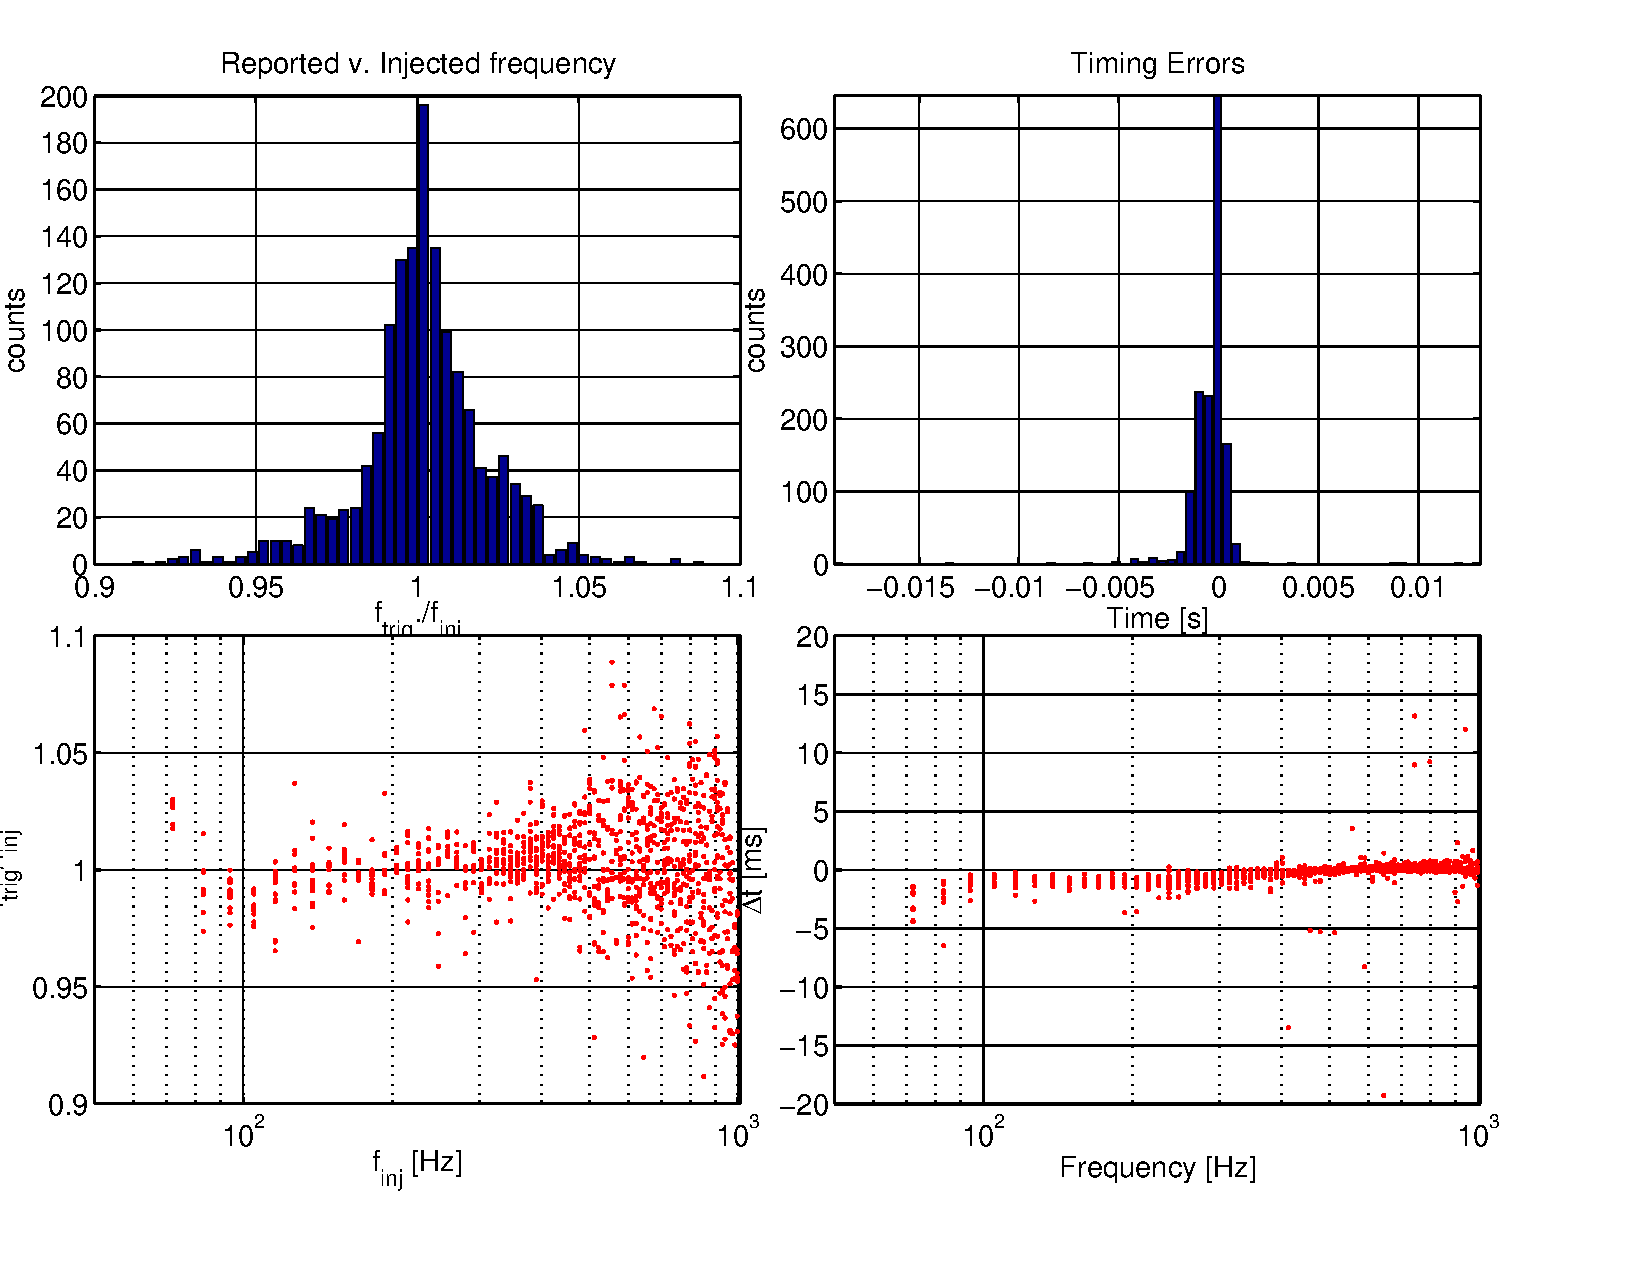
\includegraphics[angle=0,width=6.5in]{Figures/Chap7/ParamEst-Ave.pdf}}
\caption[Parameter Estimation]{Parameters reported by the pipeline versus the 
         injected parameters. In this plot the 'loudest' 10\% of the triggers
         for each event are used to estimate the trigger parameters by doing 
         an (SNR)$^2$ weighted average.}
\label{fig:ParamEst}
\end{figure}


\subsubsection{Detection Efficiency}

To interpret the results of the analysis, we measure the detection efficiency
of the software injected signals. As shown
in Figures~\ref{fig:L1efficiency} and \ref{fig:H1efficiency}, we detect almost 
all of the high SNR events and none of the low SNR
events. There is a gradual increase in the probability of detecting a signal
as the SNR is increased, which we have fit to a sigmoid function~\cite{S1:Bursts}:

\begin{figure}[!h]
\centerline{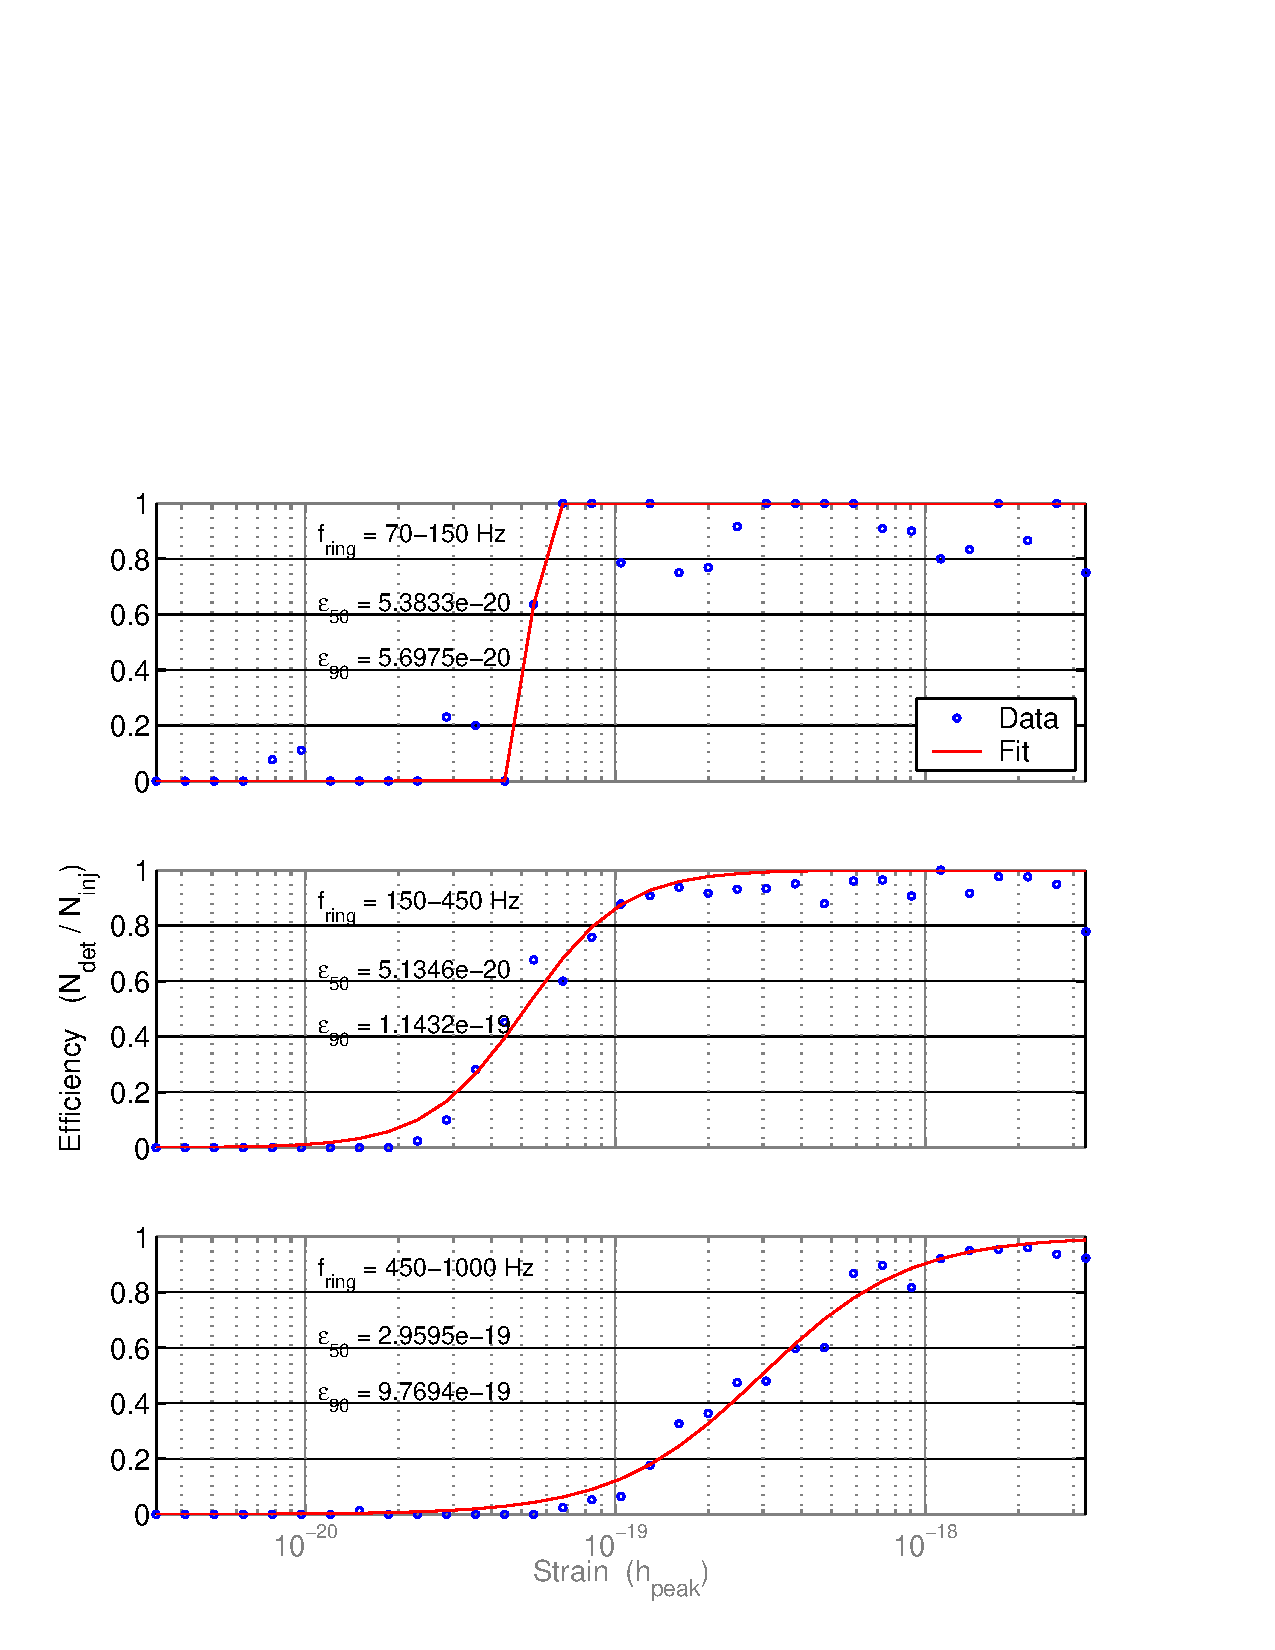
\includegraphics[angle=0,height=7in]{Figures/Chap7/eff-L1.pdf}}
\caption[L1 Detection Efficiency]{Detection efficiency of L1 as a function of peak strain. 
         The three plots show the results in 3 frequency bands. Also indicated are the 
         50\% and 90\% efficiency levels corresponding to a 50\% and 10\% false dismissal 
         probability, respectively.}
\label{fig:L1efficiency}
\end{figure}

\begin{figure}[!h]
\centerline{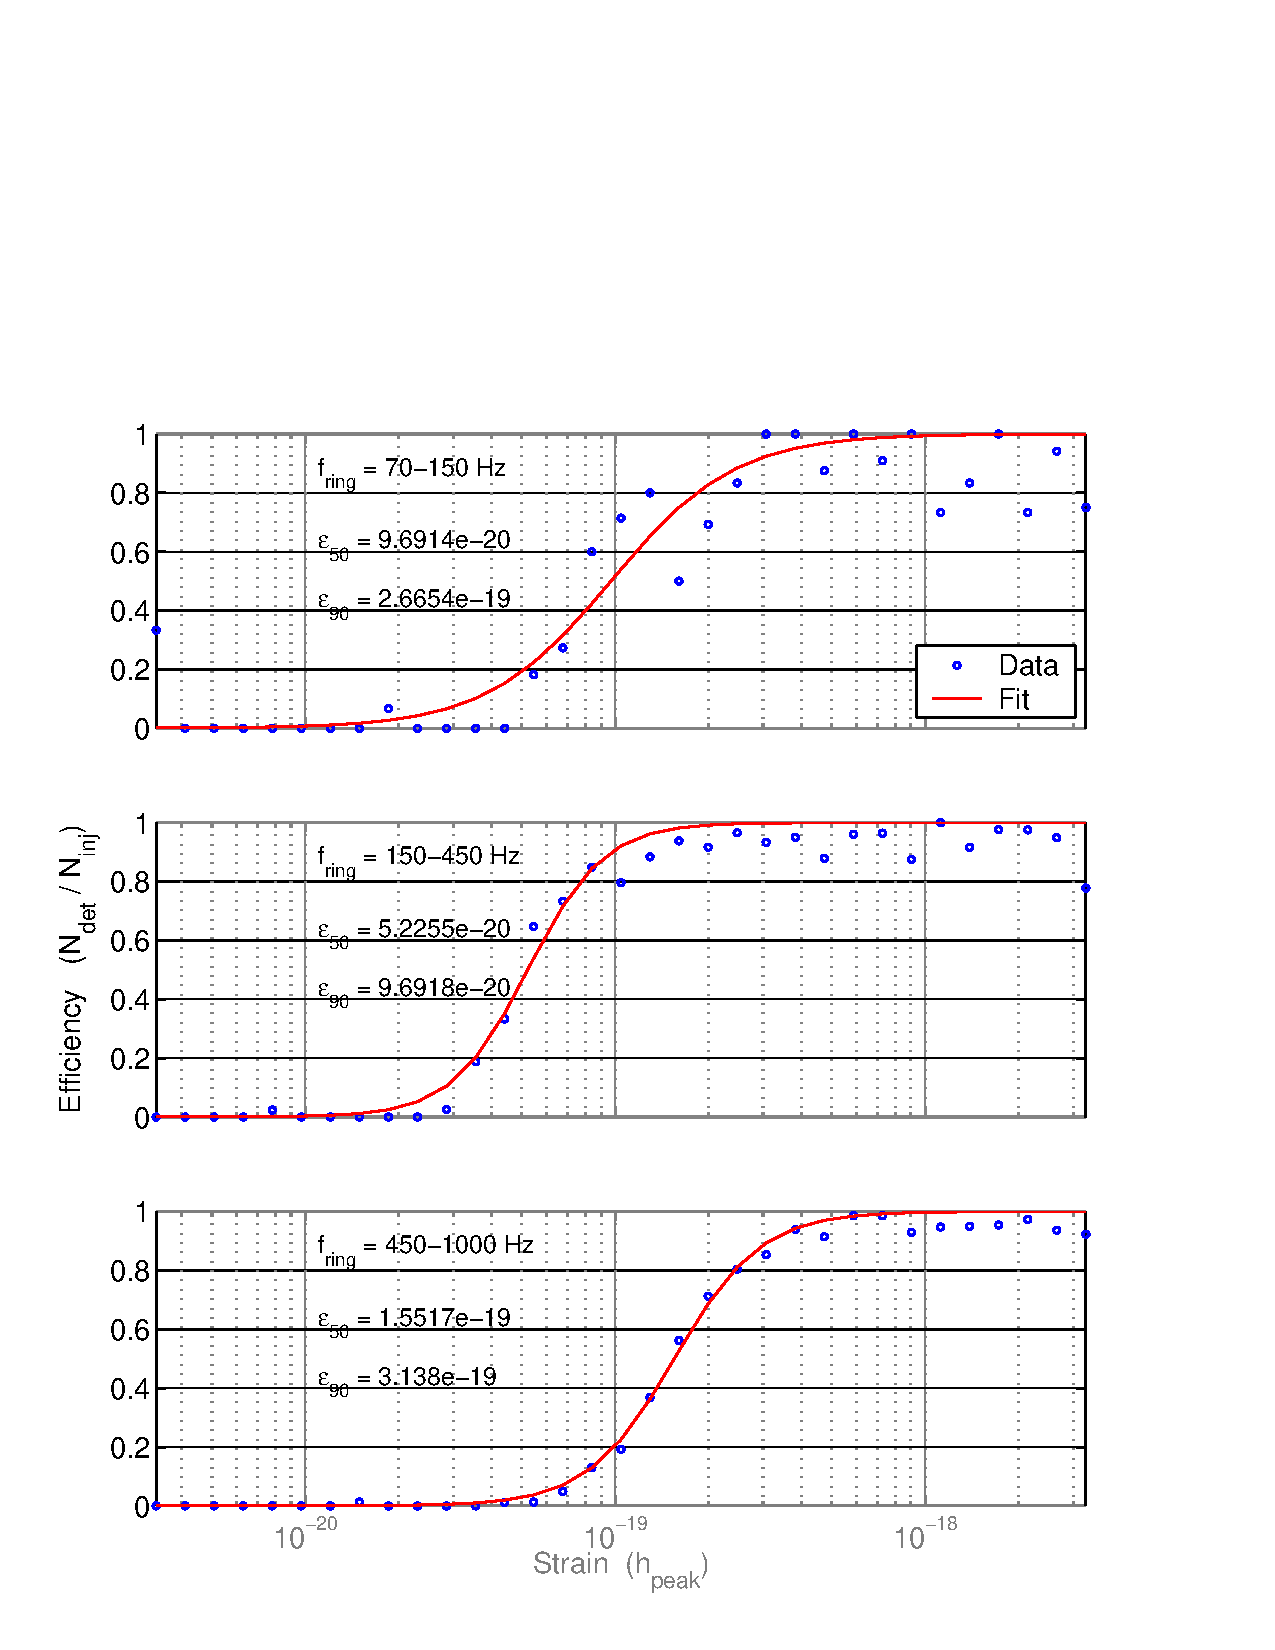
\includegraphics[angle=0,height=7in]{Figures/Chap7/eff-H1.pdf}}
\caption[H1 Detection Efficiency]{Detection efficiency of H1 as a function of peak strain. 
         The three plots show the results in 3 frequency bands. Also indicated are the 
         50\% and 90\% efficiency levels
         corresponding to a 50\% and 10\% false dismissal probability, respectively.}
\label{fig:H1efficiency}
\end{figure}

\begin{equation}
E(h) = \left[1 + exp(-\frac{log_{10}(h)-log_{10}(h_{50})}{a})\right]^{-1}
\end{equation}
We call the point at which there is a 50\% probability of detection,
$\epsilon_{50}$. This $\epsilon_{50}$, in terms of strain, is a function also
of frequency and Q.


\subsection{Hardware Injections}
\label{sec:HI}

Signals are also injected in real time via hardware; more to test the realism of the
software injections than anything else. The signals are calculated ahead
of time and saved into a file. The file is then loaded and the waveform is
injected into the number stream driving the longitudinal degree of freedom
of the optic. The injection point is labeled as 'EXC' in the ETMX path on 
the right hand side of Figure~\ref{fig:LSCscreen}.

Figure~\ref{fig:strainer} shows the amplitude of the injected ringdowns
compared with the noise in the detectors.

\begin{figure}[!h]
\centerline{\includegraphics[angle=0,width=6.5in]{Figures/Chap7/strainer.pdf}}
\caption[Injection Amplitudes]{The peak amplitudes of the hardware injections
         are plotted versus the noise, $h_{rms} = \sqrt{f S_h(f)}$ for the 
         three interferometers during the S2 Science Run.}
\label{fig:strainer}
\end{figure}
Comparison between the hardware and software injections is ongoing.


\section{Results}

The entire pipeline was then run on all the H1-L1 double coincident segments.
The run was done with a SNR threshold of 6 on L1 and a threshold of 5 on H1.


\subsection{Distribution of triggers}

Figures \ref{fig:hist_bands} and \ref{fig:hist_f} show the distribution
of the triggers from the individual interferometers.

\begin{figure}[!h]
\centerline{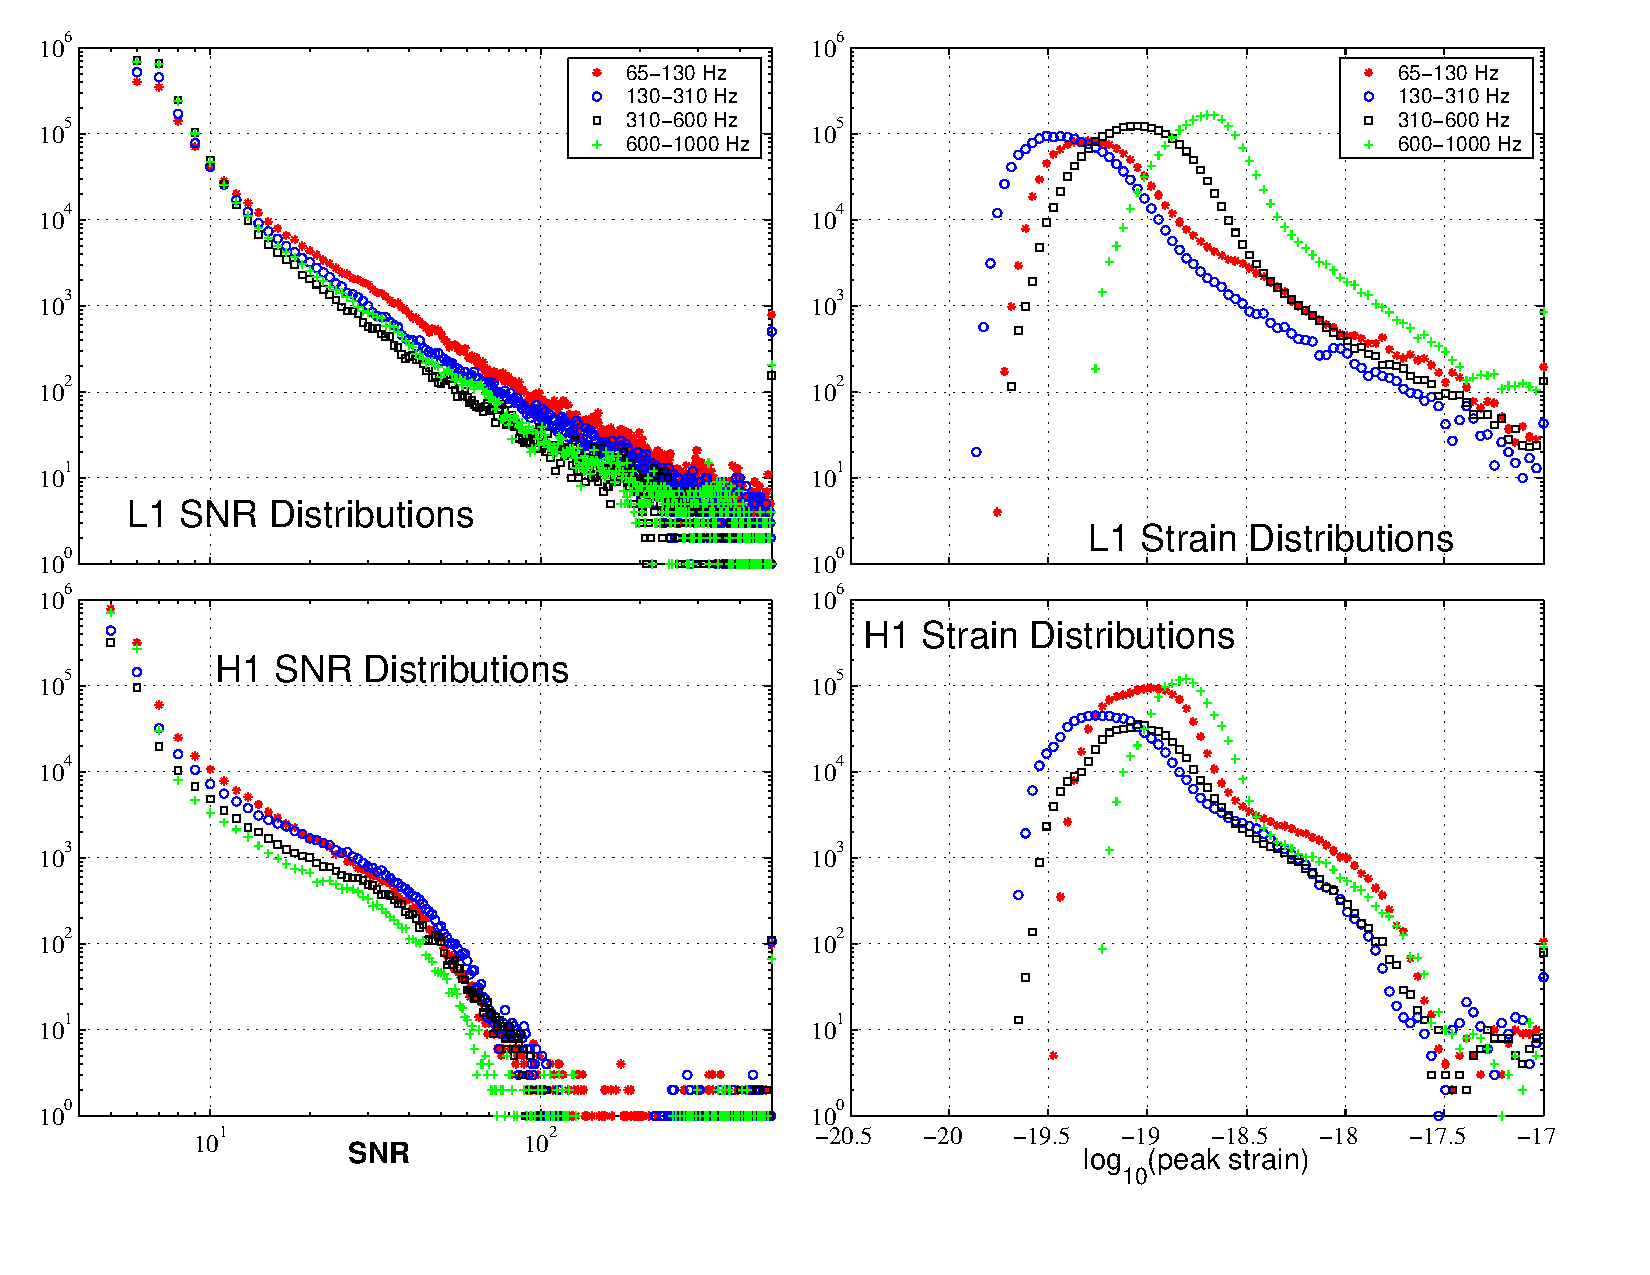
\includegraphics[angle=0,width=6.5in]{Figures/Chap7/cooter.pdf}}
\caption[Histograms of the Bands]{Amplitude distribution of the triggers in
         four separate bands. The choice of bands was made to highlight the
         different noise character in the different bands.}
\label{fig:hist_bands}
\end{figure}


\begin{figure}[!h]
\centerline{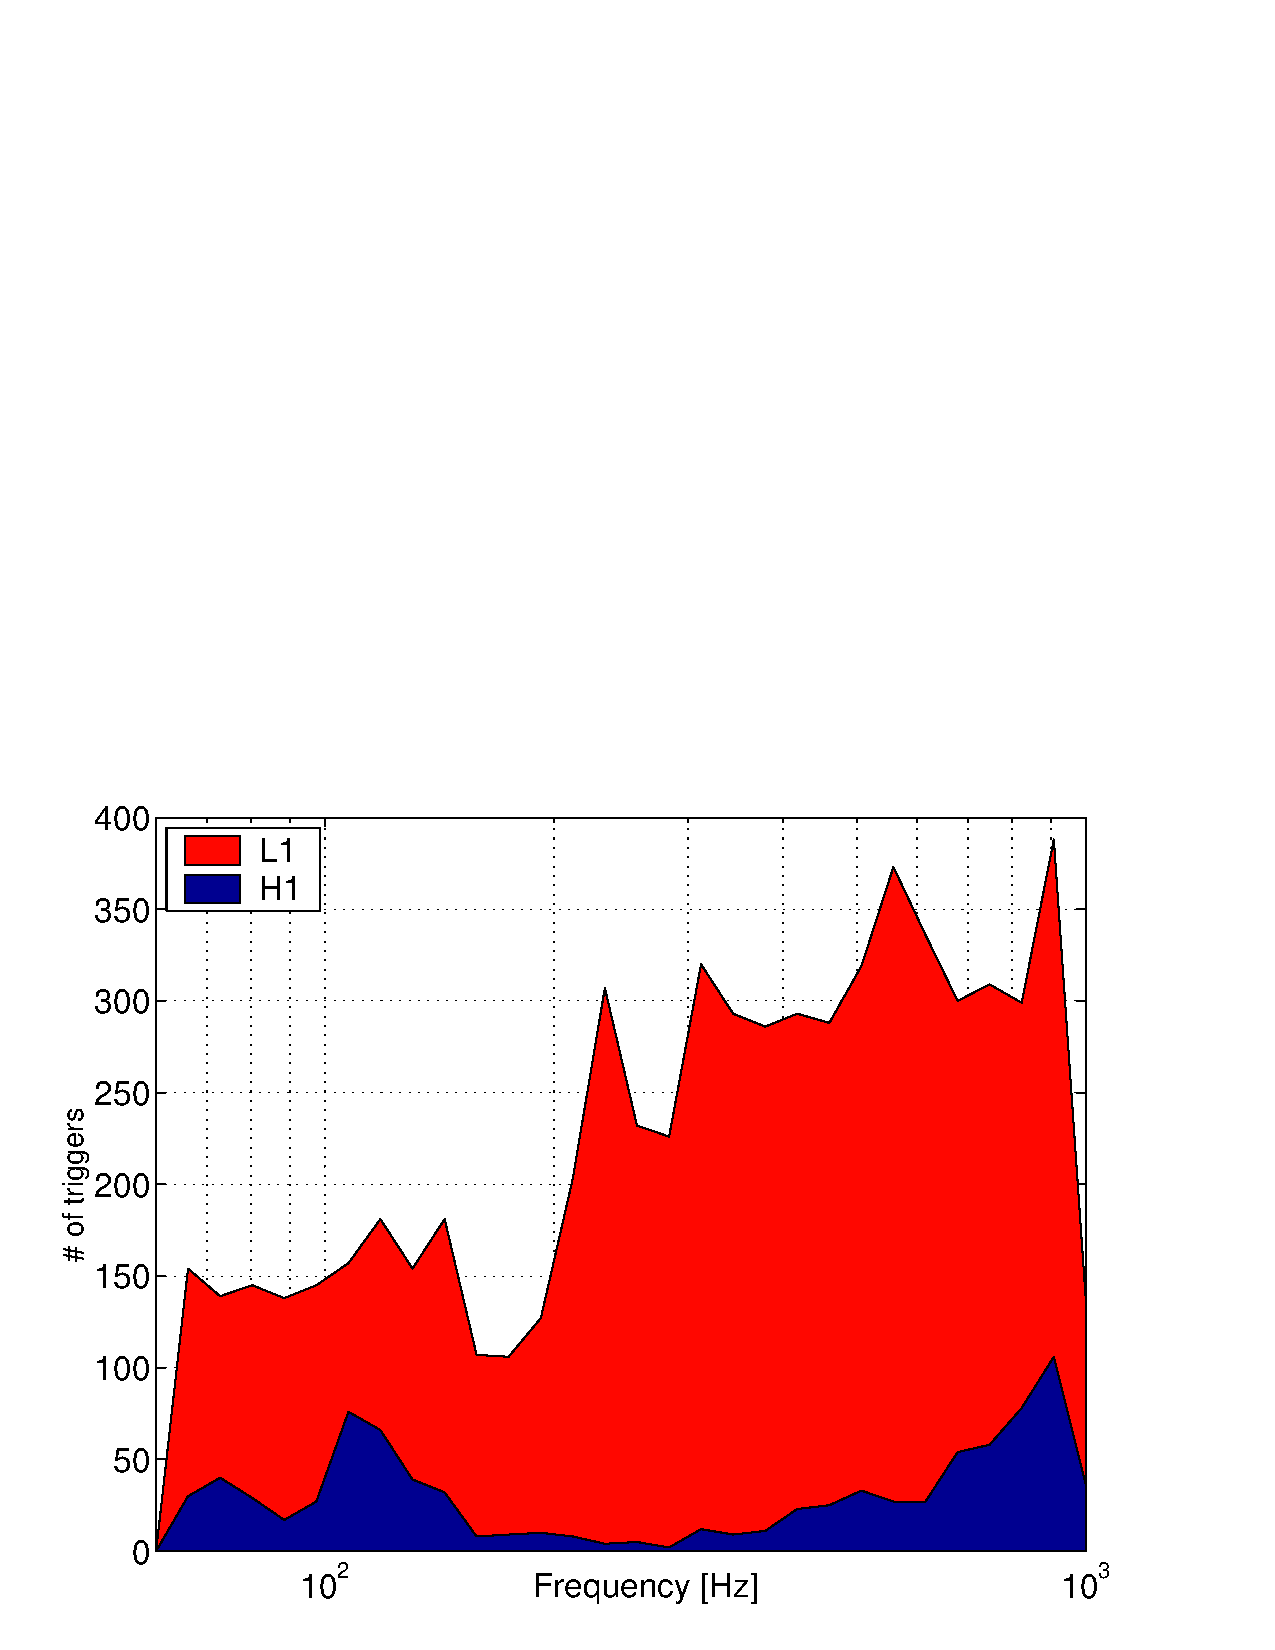
\includegraphics[angle=0,width=6.5in]{Figures/Chap7/f_hist_all.pdf}}
\caption[Number of triggers v. Frequency]{The total number of triggers per frequency
         binned logarithmically. The total number of triggers in any bin is dominated
         by the large population of low SNR events.}
\label{fig:hist_f}
\end{figure}



\subsection{Coincident Events}
After applying the coincidence criteria listed in Section~\ref{sec:coin_anal} 
there will be some remaining events; how many depends on the threshold used. 
Figure~\ref{fig:ce_hist} shows the distribution of the (L1) SNR of the 
coincident events after clustering in 100 ms chunks.

\begin{figure}[!h]
\centerline{\includegraphics[angle=0,width=6.5in]{Figures/Chap7/co_dist.pdf}}
\caption[Histogram of Coincidences]{SNR Distribution of clustered coincident events
         with SNR $<$ 50}
\label{fig:ce_hist}
\end{figure}
Since the character of the instrument noise is not Gaussian, it is difficult to 
tell if the non-Gaussian outliers are signal or noise.
 
To see if there are a statistically significant number of coincident
events within the time window determined by the light travel time
between the detectors, we re-ran the coincidence analysis many times, 
each time inserting a pseudo-random time shift in the triggers of 
one of the interferometers. Figure~\ref{fig:timelag} shows an 
example of one of these time lag simulations.

If there had been a number of real events (noise or otherwise) which were
coincident between detectors, then one would
expect there to be an excess of triggers at a lag of zero seconds. At various
thresholds and with many choices of frequency bands, there are no excess
coincident events above the level of one standard deviation above the
background.

\begin{figure}[!h]
\centerline{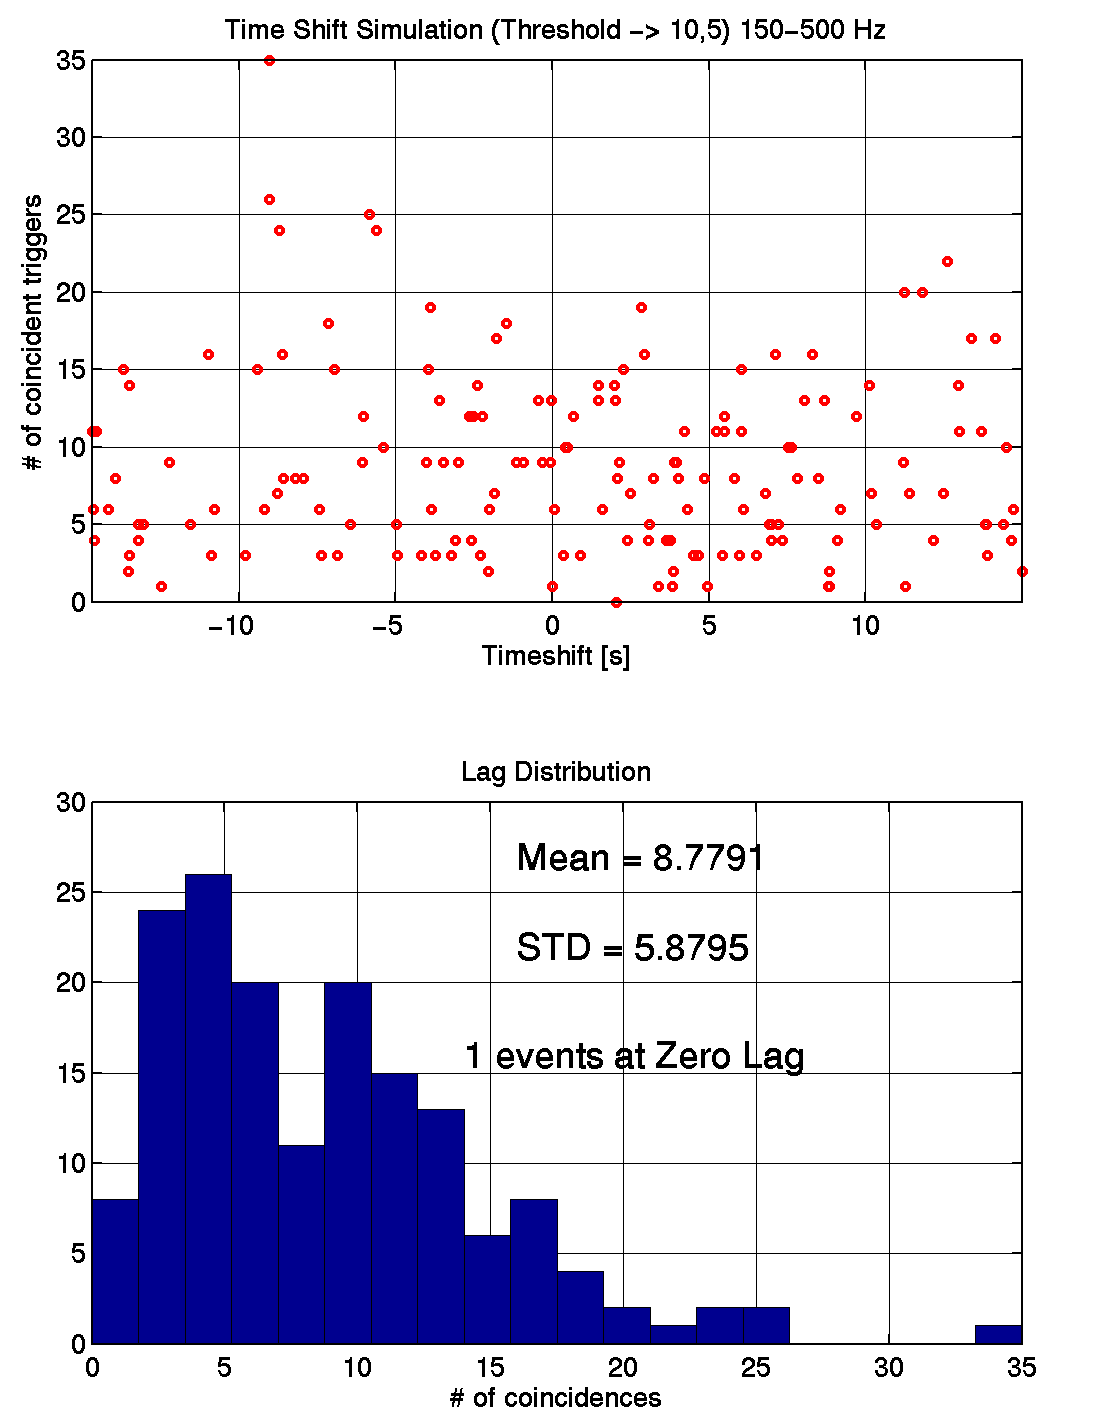
\includegraphics[angle=0,height=6.5in]{Figures/Chap7/lag_mid_dist.png}}
\caption[Time Lags]{Upper plot shows the number of coincident events as a
         function of artificial time lag between the interferometers. The
         lower plot shows the distribution of the upper plot. Both plots
         include only the triggers from the sensitive 150-500 Hz region. The
         L1 threshold = 10 and the H1 threshold = 5.}
\label{fig:timelag}
\end{figure}
The same plot as in Figure~\ref{fig:timelag} was made for several other choices
of threshold and frequency band, always with similar results: the number of
events at zero lag are always within 1 $\sigma$ of the background.

From these time shift plots, we can see that there is nothing special about the 
events at zero lag. In the most sensitive band (150-500 Hz), there are no
coincident events above an SNR of 9, except for two instrumental artifacts.


\section{Examination of the Remaining Coincidences}

This section looks at the coincident events at zero lag. Each event is tagged with
an event \# in Table~\ref{t:Events}.

\begin{table}[!h]
\begin{center}
\begin{tabular}{|c|c|c|c|c|c|c|}
\hline
\multicolumn{7}{|l|}
{{\bf \textsf{Event Triggers}}}\\ \hline \hline

Event \# & GPS Start Time & SNR & Strain (h$_{\mbox{peak}}$) & f &  Q & Note \\ \hline \hline

1    &  729434662.741  &    12   &   8.9e-20    &      84   &     2  & ---      \\ \hline
2    &  729531388.721  &    16   &   1.5e-19    &      78   &    17  & 60 Hz    \\ \hline
3    &  729541448.431  &    10   &   4.7e-19    &     803   &     6  & ---      \\ \hline
4    &  729920354.113  &    15   &   2.0e-19    &      65   &    21  & 60 Hz    \\ \hline
5    &  730094894.358  &    11   &   1.4e-19    &     566   &    21  & ---      \\ \hline
6    &  730133435.403  &   152   &   7.3e-18    &     994   &    21  & ADC      \\ \hline
7    &  730137174.219  &    16   &   5.0e-19    &     690   &    21  & Vio$^2$  \\ \hline
8    &  730284595.603  &    17   &   2.4e-19    &      65   &     3  & 60 Hz    \\ \hline
9    &  730285409.016  &    12   &   8.6e-20    &      94   &    18  & ---      \\ \hline
10   &  730443122.214  &    12   &   7.3e-20    &      91   &    21  & ---      \\ \hline
11   &  730443379.098  &    36   &   2.9e-19    &      80   &    11  & 60 Hz    \\ \hline
12   &  730462872.134  &    30   &   1.7e-19    &      83   &    21  & SNR       \\ \hline
13   &  730528198.849  &    13   &   8.7e-20    &      97   &    11  & ---      \\ \hline
14   &  730528295.260  &    13   &   6.2e-20    &     118   &    21  & ---      \\ \hline
15   &  730570357.681  &    11   &   2.5e-19    &     637   &    14  & ---      \\ \hline
16   &  730581701.429  &    12   &   5.0e-20    &     135   &    21  & ---      \\ \hline
17   &  730592358.344  &    12   &   8.0e-20    &      87   &    11  & ---      \\ \hline
18   &  730605715.704  &    10   &   3.7e-20    &     136   &    21  & ---      \\ \hline
19   &  730669046.827  &    10   &   1.0e-19    &      80   &    21  & ---      \\ \hline
20   &  730881699.750  &   132   &   4.7e-19    &     180   &    21  & ADC      \\ \hline
21   &  732581991.246  &  1580   &   5.4e-17    &     734   &    11  & ADC      \\ \hline
22   &  732637065.650  &    11   &   7.7e-20    &     119   &    11  & ---      \\ \hline
23   &  732639925.100  &    14   &   5.0e-19    &     848   &    17  & ---      \\ \hline
24   &  733037033.244  &    71   &   6.1e-19    &     353   &    21  & Violin   \\ \hline
25   &  733037804.016  &    15   &   6.4e-20    &     112   &    21  & ???      \\ \hline
26   &  733592255.881  &    11   &   2.4e-19    &     695   &    21  & ---      \\ \hline
27   &  733749193.282  &    13   &   2.1e-19    &     669   &    18  & ---      \\ \hline
28   &  733751635.889  &    15   &   7.8e-20    &      78   &    21  & ---      \\ \hline
29   &  734139127.398  &    13   &   8.5e-20    &      78   &    16  & ---      \\ \hline
30   &  734149435.240  &    12   &   5.8e-20    &      94   &    21  & ---      \\ \hline 
\end{tabular}
\end{center}
\caption[Coincident Events in S2]{Parameters for the coincident events in S2 with
                                  SNR $>$ 10}
\label{t:Events}
\end{table}

\subsection{Study of the Remaining Events}

The coincident events with a SNR in L1 above 10 were examined 'by hand'
by looking at the time series plots after bandpassing the data in a few hundred Hz
band around the trigger's central frequency.


\subsubsection{Event \#21 - SNR = 1580}

Event \#21 is an ADC saturation. The AS\_Q time series that we record is a digitally
processed version of the raw ADC inputs. To determine what the ADC recorded we apply
the inverse of that digital processing. Applying this procedure to \#21 we see that the
ADC signal suddenly rails several times at +32767 and -32768. The signal then recovers
and the interferometer resumes normal operation.

During the course of the run several of these events were observed and more often than
not these saturations caused a loss of lock. This was tracked down to be a malfunctioning
piece of electronics; voltage noise on the gain control of the AS port whitening board
caused fast steps in the AS\_Q ADC signal. 

Following the S2 run, software monitors were put in place to record all ADC saturations
and the flagged data have been vetoed. Even better, a new design for the whitening 
electronics uses a TTL logic control for the gain command, eliminating this type of 
malfunction.


\subsubsection{Event \#6 - SNR = 152}

This one is another ADC saturation, although of a different nature. Just below the
sensitive 70-1000 Hz band is a large 'wall' of noise which is of a seismic nature,
although not the standard seismic coupling mechanism. It comes from a variety of noise
sources including mechanical resonances of the optical lever piers, unfiltered
electronics noise from the wavefront sensors, and in this case, nonlinear upconversion
of the $\sim$ bounce mode of a suspended large optic. During the run, we noticed that
ground noise due to some malfunctioning HVAC equipment would excite the mechanical
modes of several optics. Large amplitude signals (through some unknown mechanism)
would also produce a large component at 3$\times$ the fundamental frequency. This
large signal at $\sim$35 Hz is then amplified by the analog whitening filter.

The RMS from this signal is several times smaller than the ADC range, but statistically
we expect to see a large excursion once in awhile. These excursions can either cause
a loss of lock or, as in this case, produce a strong glitch.

Based on these experiences, a new whitening filter design was implemented before the
next science run. The new whitening filter has $\sim 4 \times$ less gain in this
noisy band. In addition, there are some efforts to fix noisy HVAC equipment.


\subsubsection{Event \#20   SNR = 132}

Another ADC saturation. Essentially the same behavior as Event \#6.


\subsubsection{Event \#24   SNR = 71   f = 353 Hz}

Nothing in H1. A sudden sharp transient in L1. The template frequency
is the same as that of one of the test mass violin modes, but it is not
clear if this is a coincidence or not.


\subsubsection{Event \#11   SNR = 36  f = 80 Hz}

Looks like some transient upconversion around 60 Hz. It is only a small
increase in the RMS of the 60 Hz shoulders; this is a common occurrence
and this $\sim$20 Hz band around 60 and 120 Hz often show this
non-stationary behavior.


\subsubsection{Event \#12   SNR = 30  f = 83 Hz}

Interesting looking glitch in L1, but at too low of a level to show up
in the bandpassed H1 or H2 time series.

\subsubsection{Event \#8   SNR = 17   f = 65 Hz}

Just like \#11. 60 Hz junk.


\subsubsection{Event \#7   SNR = 16   f = 690 Hz}

A random fluctuation in the 2nd harmonic of a violin mode in both interferometers.
It seems like the data in a small band around the first and second violin mode
harmonics is constantly getting rung up. If this cannot be suppressed by
further notching in the control servos, it may be necessary to ignore all the
triggers from these bands.


\subsubsection{Event \#2   SNR = 16   f = 78 Hz}

L1 AS\_Q goes to +/- 20000 ADC counts but does not saturate. Looks like a
35 Hz and 60 Hz problems evident in events \#6 and \#11.


\subsubsection{Event \#4   SNR = 15   f = 65 Hz}


\subsubsection{Event \#25   SNR = 15   f = 112 Hz}

There is nothing visible in the time series above the background.



\section{Future Improvements}

This analysis is a preliminary attempt to look for ringdown signals with the
main emphasis being on uncovering gross problems or difficulties. As such,
there a number of ideas / methods / techniques which were not implemented
yet but are listed here for posterity.

\begin{itemize}

\item It seems clear that the burden is on the commissioning team to
      reduce the large variability in the noise floor and the high rate 
      of transients. A noble goal would be to reduce the rate of transients
      until the random double coincident rate meets the expectations from
      Poisson statistics up to SNR$= 15$. Efforts are underway to develop 
      a 'ringdown' monitor
      program to run in the control room at both sites to give a feel for
      the variability of the false rate as instrument parameters are adjusted
      during commissioning of the interferometer.

\item A method needs to be developed to veto non-ringdown events which cause
      the templates to exceed threshold. One method may be examining the software 
      injections to determine the amplitude and start times in neighboring
      templates\cite{Jolien:40m}. A true ringdown signal should have a well 
      defined distribution
      in template space. One has to be careful not to veto a potential
      merger-ringdown signal by placing too tight a criteria.

\item Do a direct waveform consistency check by cross-correlating the
      interferometer outputs in the neighborhood of the events. This is
      a technique currently being developed for detecting unmodeled 
      bursts~\cite{Laura:Rstat}.

\item Do a real Monte-Carlo simulation over the matched filter and 
      coincidence parameters to optimize the search sensitivity.

\end{itemize} 


\section{Conclusions}

A preliminary search was done for damped sinusoids in the data. The search
highlighted several problems in the interferometers and in the search method.

The equivalent strain amplitude of the coincident events at SNR of 10
agrees with the rough estimate made by comparison with noise spectral density.

It is clear that more simulations will have to be done to determine precisely
the detection efficiency as a function of time for each interferometer. A method
of vetoing the non-ringdown triggers needs to be developed to reduce the
false rate.






